\chapter{Backgrounds in classification and detection architectures}
\label{chap:ch3}

In the interest of improving image classification, there have been many models documented, each trying to be better than the previous ones. The most commonly used include ResNet, DenseNet, VGGNet, AlexNet and GoogLeNet ~\cite{link8}. The same can be said about detection models; some of the most popular in 2024 are YOLO (You Only Look Once), RetinaNet, Faster-RCNN and EfficientDet~\cite{carte11}.

Of all of these models, I chose to integrate into my system GoogLeNet for classification and EfficientDet for detection.

\section{GoogLeNet Architecture}

This models first appereance was in an research paper published in 2014 called "Going Deeper with Convolutions" ~\cite{carte13}. The researches at Google, along with other universities, received that year the first place in the  ILSVRC 2014 image classification competition, by achieving a less error rate than the other contestants. They managed this by introducing new concepts, such as 1x1 convolution, global average pooling, inception module and auxiliary classifiers. Table \ref{tab:tab11} shows the distribution of the layers in the GoogLe Net architecture.

\begin{table}[H]
    \centering
    \resizebox{\textwidth}{!}{%
    \begin{tabular}{|c|c|c|c|c|c|c|c|c|c|c|c|}
        \hline
        Type & Path size/Stride & Output size & Depth & \#1x1 & \#3x3 reduce & \#3x3 & \#5x5 reduce & \#5x5 & pool proj & params & ops\\
        \hline \hline
        Convolution & 7x7/2 & 112x112x64 & 1 & & & & & & & 2.7K & 34M \\
        \hline
        Maxpool & 3x3/2 & 56x56x64 & 0 & & & & & & & & \\
        \hline
        Convolution & 3x3/1 & 56x56x192 & 2 & & 64 & 192 & & & & 112K & 360M\\
        \hline
        MaxPool & 3x3/2 & 28x28x192 & 0 & & & & & & & & \\
        \hline
        Inception(3a) & & 28x28x256 & 2 & 64 & 96 & 128 & 16 & 32 & 32 & 159K & 128M \\
        \hline
        Inception(3b) & & 28x28x480 & 2 & 128 & 128 & 192 & 32 & 96 & 64 & 380K & 304M \\
        \hline
        Maxpool & 3x3/2 & 14x14x480 & 0 & & & & & & & & \\
        \hline
        Inception(4a) & & 14x14x512 & 2 & 192 & 96 & 208 & 16 & 48 & 64 & 364K & 73M \\
        \hline
        Inception(4b) & & 14x14x512 & 2 & 160 & 112 & 224 & 24 & 64 & 64 & 473K & 88M \\
        \hline
        Inception(4c) & & 14x14x512 & 2 & 128 & 128 & 256 & 24 & 64 & 64 & 463K & 100M \\
        \hline
        Inception(4d) & & 14x14x528 & 2 & 112 & 144 & 288 & 32 & 64 & 64 & 580K & 119M \\
        \hline
        Inception(4e) & & 14x14x832 & 2 & 256 & 160 & 320 & 32 & 128 & 128 & 840K & 170M \\
        \hline
        Maxpool & 3x3/2 & 7x7x832 & 0 & & & & & & & & \\
        \hline
        Inception(5a) & & 7x7x832 & 2 & 256 & 160 & 320 & 32 & 128 & 128 & 1072K & 54M \\
        \hline
        Inception(5b) & & 7x7x1024 & 2 & 384 & 192 & 384 & 48 & 128 & 128 & 1388K & 71M \\
        \hline
        Avgpool & 7x7/1 & 1x1x1024 & 0 & & & & & & & & \\
        \hline
        Dropout(40\%) & & 1x1x1024 & 0 & & & & & & & & \\
        \hline
        Linear & & 1x1x1000 & 1 & & & & & & & 1000K & 1M \\
        \hline
    \end{tabular}}
    \caption{Layer structure of the GoogLeNet architecture}
    \label{tab:tab11}
\end{table}

\subsection{1x1 convolution layer}

The use of 1$\times$1 convolution reduces the overall number of parameters of the model ~\cite{link17}. The effect of this operation is increasing the depth of the model, which can help catch and understand complex patterns in the input images. Images \ref{fig:fig42} showcase how many parameters result from a 5$\times$5 convolution without a 1$\times$1 convolution as intermediate compared to one with the 1$\times$1 convolution. 

\begin{figure}[H]
    \subfigure[Without intermediate]{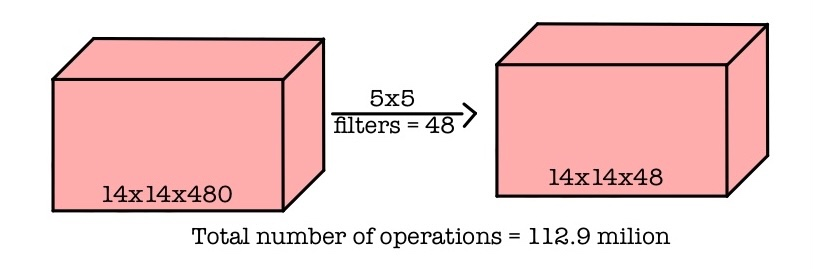
\includegraphics[width=0.45\linewidth]{figures/Figure55.png}}
    \subfigure[With intermediate]{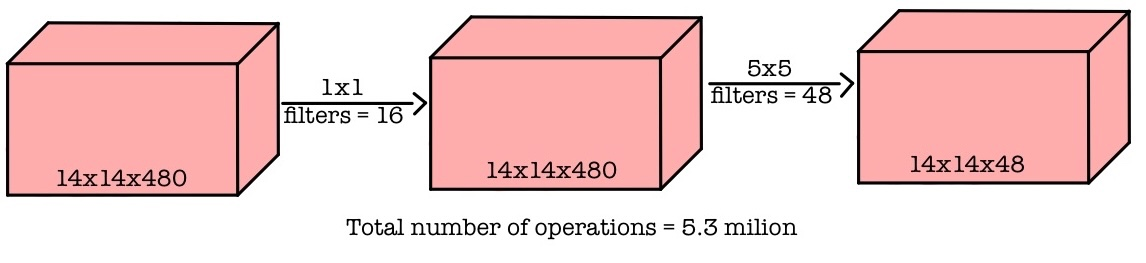
\includegraphics[width=0.45\linewidth]{figures/Figure56.png}}
    \caption{Difference in parameters between convolution operations}
    \label{fig:fig42}
\end{figure}

\subsection{Global Average Pooling}

This method is also a method of decreasing the number of trainable parameters, which then reduces computation costs. Other architectures place their fully connected layers at the end of the network, which contain the largest number of parameters. To combat this, GoogLeNet proposes the global average pooling method, also used at the end of network, which takes a 7$\times$7 feature map and reduces it to 1$\times$1. Along with reducing the number of trainable parameters, this also increases accuracy by 0.6\%~\cite{link17}. 

\subsection{Inception Module}

While GoogLeNet is not the first architecture to use inception modules in it's configuration, it is the first to set the convolution size for each layer. In these modules, 1$\times$1, 3$\times$3 and 5$\times$5 along with 3$\times$3 max pooling layers are performed in parallel at the input, while the output of these convolutions are stacked in order to obtain one final output. The idea behind this is that convolution layers of different filter sizes will manage objects at multiple scales better ~\cite{link17}. Image \ref{fig:fig43} provides two examples of possible inception module concepts, n\"aive approach and the reduced dimensions one, the latter of which is used in the GoogLeNet architecture.

\begin{figure}[H]
    \centering
    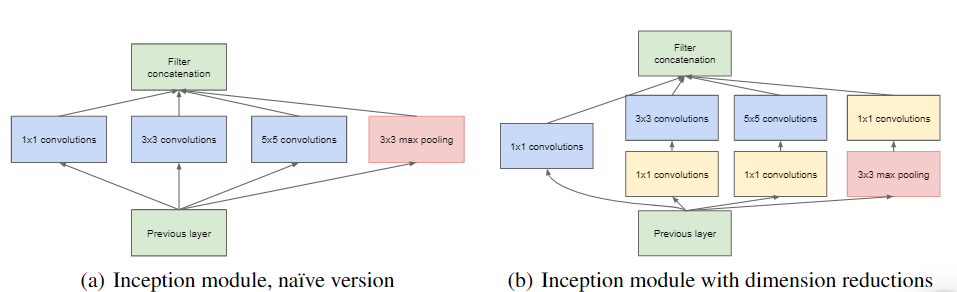
\includegraphics[width=1\linewidth]{figures/Figure57.png}
    \caption{Difference between the two main concepts of the inception module, obtained from ~\cite{carte13}}
    \label{fig:fig43}
\end{figure}

The main purpose of this second concept, employed by the GoogLeNet architecture is overall reduction of parameters. Adding the reduction of dimensions provides a 60\% decrease in number of parameters~\cite{carte14}.

\subsection{Auxiliary Module}

These modules, two in total, are used only during the training stage of the model. They help in combating gradient vanishing problem and providing regularization.

\section{EfficientDet Architecture}

The EfficientDet model is a new family of object detectors based on two main optimizations, those being efficient multi-scale feature fusion and model scaling. Along with those optimizations, different models have been tested to serve as the backbone of the model, and for this particular model, EfficientNet has proven to be a sufficient backbone architecture~\cite{carte8}.

The first challenge of this model was feature fusion, a concept introduced to aid convolutional neural networks in identifying objects from images when the objects' sizes are either too small or exceed the convolutional kernel's receptive field.~\cite{carte9}. It has been discovered that changing the resolution of the image solved the sensitivity that neural networks have to the images' size, to some extent, as shown in figure \ref{fig:fig4}.

\begin{figure}[!ht]
    \centering
    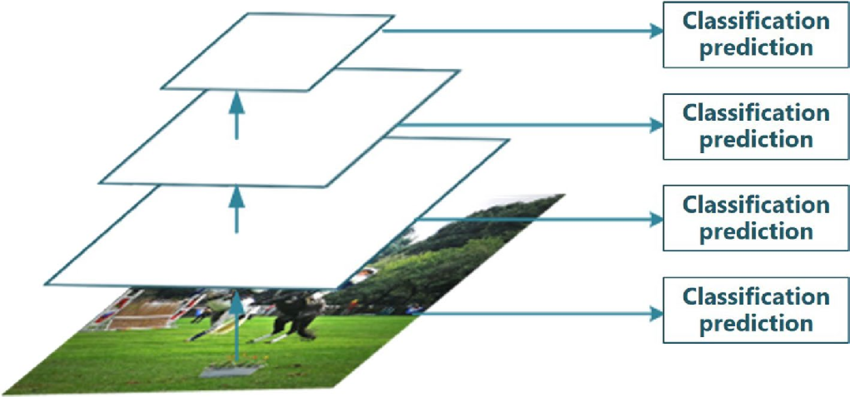
\includegraphics[width=0.7\textwidth]{figures/Figure4.png}
    \caption{Pattern diagram of image pyramid, obtained from ~\cite{link13}}
    \label{fig:fig4}
\end{figure}

The problem with this discovery was that the cost of system storage for creating a pyramid of the same image in different resolutions and computational resources are too harsh, therefore deeming this method rarely usable. Because each resolution had its advantages, a way to combine features from high-resolution features of shallow networks with the high-level semantic information of high-level network features was researched. Thus, the FPN, or Feature Pyramid Network, has been used to extract from deep-layer networks and get the same features as the shallow-layer features by up-sampling, as shown in figure \ref{fig:fig5}. 

\begin{figure}[!ht]
    \centering
    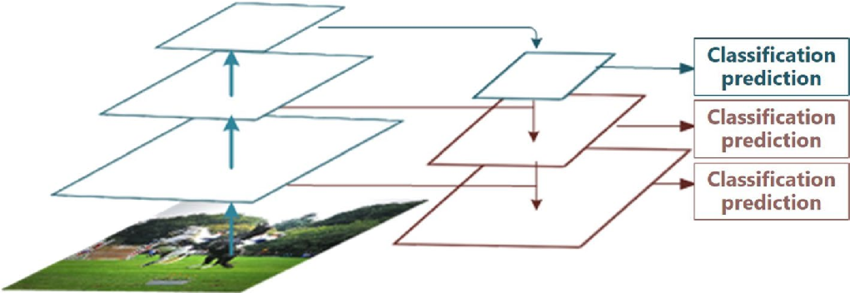
\includegraphics[width=0.7\linewidth]{figures/Figure5.png}
    \caption{Pattern diagram of feature pyramid network, obtained from ~\cite{link12}}
    \label{fig:fig5}
\end{figure}

In this particular model, a BiPFN has been introduced, Bi-directional FPN, which utilizes learnable weights to learn the importance of different input features from different resolutions.

The second challenge is model-scaling. This method was popularized in \cite{carte10}, and is used to uniformly scale all dimensions of depth, width and resolution using a compound coefficient. This scaling method, called compound scaling, is looking at how the different dimensions interact with each other and scales them accordingly. For the EfficientDet architecture, this scaling method is used to scale up resolution, width and depth for all layers of the backbone, BiFPN and the bounding boxes and classification network.

Finally, for the backbone, EfficientNet has been observed to achieve better accuracy than other previously used backbones ~\cite{carte8}. 
% \subsubsection{Bi-directional Feature Pyramid Network}
The baseline strategy for a standard FPN is to aggregate the features from the different levels of resolution in a top-down manner, from the features of the image with the lowest resolution to the ones from the highest one. For example, if a feature is extracted from the lowest resolution image, that feature is passed through a convolutional layer, used for feature processing, and the resulting output is then resized, which could be upsampling or downsampling in order to match the resolution of the following feature and so on ~\cite{carte8}.

The conventional FPN is, however, limited by the one-directional feature flow. To correct this use, PANet, or Path Aggregation Network, is introduced and adds a path going bottom-up. These methods are still not ideal because of the cost of computations and parameters needed. The strategy proposed in \cite{carte8} says that nodes that have only one edge going into them should be removed because the lack of multiple input edges corresponds to less contribution to the overall feature network as it does not involve feature fusion. Moreover, between every input and output node at the same level, there are edges added in order to add more feature fusion without much cost, as it is on the same level. Finally, each bidirectional path is treated as one singular layer and more layers are involved in order to achieve more high-level feature fusion, as shown in figure \ref{fig:fig6}.

\begin{figure}[!ht]
    \centering
    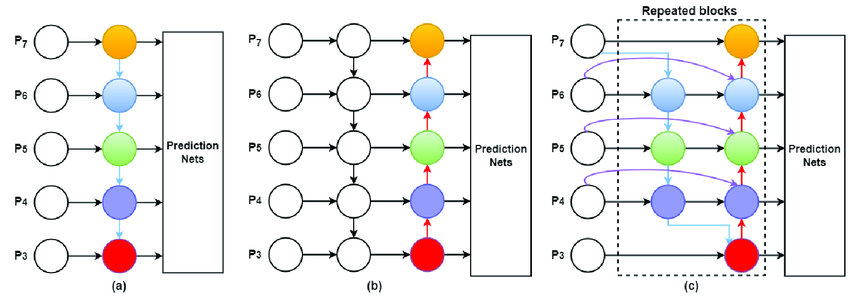
\includegraphics[width=1\textwidth]{figures/Figure6.png}
    \caption{(a)-Conventional FPN; (b)-PANet; (c)-BiFPN, obtained from ~\cite{link14}}
    \label{fig:fig6}
\end{figure}

In addition to the bidirectional cross-scale connections, the EfficientDet model takes into consideration the importance of the different features at different resolutions that can impact the predictions. Therefore, it implements a weighted feature fusion, or more precisely, a fast normalized fusion, that does not affect the performance of the GPU while also maintaining training stability~\cite{carte8}.
% \subsubsection{Conclusion}
Thus, the EfficientDet model combines all these concepts into a singular network, using ImageNet pretrained weights for the EfficientNet model, the BiFPN levels, that take the features from levels 3 to 7 from the backbone and applies feature fusion. In the end, these features are sent to a classification head and a regression head to both classify the objects detected and provide bounding boxes for them. Below is shown the EfficientDet architecture (see Figure \ref{fig:fig7}).

\begin{figure}[!ht]
    \centering
    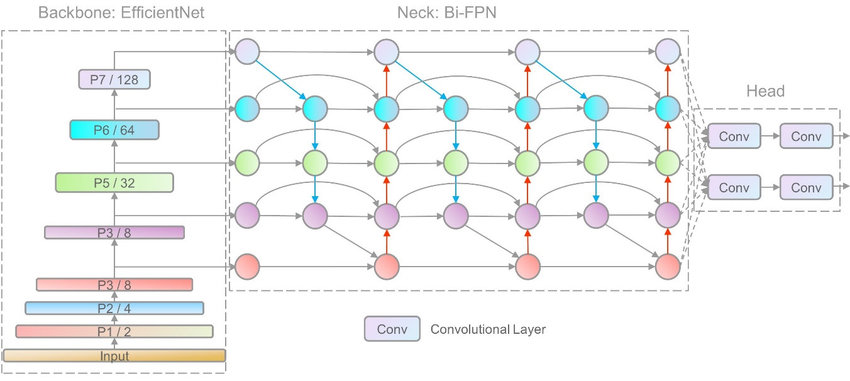
\includegraphics[width=1\textwidth]{figures/Figure7.jpg}
    \caption{EfficientDet architecture, obtained from ~\cite{link15}}
    \label{fig:fig7}
\end{figure}